% Options for packages loaded elsewhere
\PassOptionsToPackage{unicode}{hyperref}
\PassOptionsToPackage{hyphens}{url}
\PassOptionsToPackage{dvipsnames,svgnames,x11names}{xcolor}
%
\documentclass[
  letterpaper,
  DIV=11,
  numbers=noendperiod]{scrartcl}

\usepackage{amsmath,amssymb}
\usepackage{iftex}
\ifPDFTeX
  \usepackage[T1]{fontenc}
  \usepackage[utf8]{inputenc}
  \usepackage{textcomp} % provide euro and other symbols
\else % if luatex or xetex
  \usepackage{unicode-math}
  \defaultfontfeatures{Scale=MatchLowercase}
  \defaultfontfeatures[\rmfamily]{Ligatures=TeX,Scale=1}
\fi
\usepackage{lmodern}
\ifPDFTeX\else  
    % xetex/luatex font selection
\fi
% Use upquote if available, for straight quotes in verbatim environments
\IfFileExists{upquote.sty}{\usepackage{upquote}}{}
\IfFileExists{microtype.sty}{% use microtype if available
  \usepackage[]{microtype}
  \UseMicrotypeSet[protrusion]{basicmath} % disable protrusion for tt fonts
}{}
\makeatletter
\@ifundefined{KOMAClassName}{% if non-KOMA class
  \IfFileExists{parskip.sty}{%
    \usepackage{parskip}
  }{% else
    \setlength{\parindent}{0pt}
    \setlength{\parskip}{6pt plus 2pt minus 1pt}}
}{% if KOMA class
  \KOMAoptions{parskip=half}}
\makeatother
\usepackage{xcolor}
\usepackage{soul}
\setlength{\emergencystretch}{3em} % prevent overfull lines
\setcounter{secnumdepth}{-\maxdimen} % remove section numbering
% Make \paragraph and \subparagraph free-standing
\ifx\paragraph\undefined\else
  \let\oldparagraph\paragraph
  \renewcommand{\paragraph}[1]{\oldparagraph{#1}\mbox{}}
\fi
\ifx\subparagraph\undefined\else
  \let\oldsubparagraph\subparagraph
  \renewcommand{\subparagraph}[1]{\oldsubparagraph{#1}\mbox{}}
\fi

\usepackage{color}
\usepackage{fancyvrb}
\newcommand{\VerbBar}{|}
\newcommand{\VERB}{\Verb[commandchars=\\\{\}]}
\DefineVerbatimEnvironment{Highlighting}{Verbatim}{commandchars=\\\{\}}
% Add ',fontsize=\small' for more characters per line
\usepackage{framed}
\definecolor{shadecolor}{RGB}{241,243,245}
\newenvironment{Shaded}{\begin{snugshade}}{\end{snugshade}}
\newcommand{\AlertTok}[1]{\textcolor[rgb]{0.68,0.00,0.00}{#1}}
\newcommand{\AnnotationTok}[1]{\textcolor[rgb]{0.37,0.37,0.37}{#1}}
\newcommand{\AttributeTok}[1]{\textcolor[rgb]{0.40,0.45,0.13}{#1}}
\newcommand{\BaseNTok}[1]{\textcolor[rgb]{0.68,0.00,0.00}{#1}}
\newcommand{\BuiltInTok}[1]{\textcolor[rgb]{0.00,0.23,0.31}{#1}}
\newcommand{\CharTok}[1]{\textcolor[rgb]{0.13,0.47,0.30}{#1}}
\newcommand{\CommentTok}[1]{\textcolor[rgb]{0.37,0.37,0.37}{#1}}
\newcommand{\CommentVarTok}[1]{\textcolor[rgb]{0.37,0.37,0.37}{\textit{#1}}}
\newcommand{\ConstantTok}[1]{\textcolor[rgb]{0.56,0.35,0.01}{#1}}
\newcommand{\ControlFlowTok}[1]{\textcolor[rgb]{0.00,0.23,0.31}{#1}}
\newcommand{\DataTypeTok}[1]{\textcolor[rgb]{0.68,0.00,0.00}{#1}}
\newcommand{\DecValTok}[1]{\textcolor[rgb]{0.68,0.00,0.00}{#1}}
\newcommand{\DocumentationTok}[1]{\textcolor[rgb]{0.37,0.37,0.37}{\textit{#1}}}
\newcommand{\ErrorTok}[1]{\textcolor[rgb]{0.68,0.00,0.00}{#1}}
\newcommand{\ExtensionTok}[1]{\textcolor[rgb]{0.00,0.23,0.31}{#1}}
\newcommand{\FloatTok}[1]{\textcolor[rgb]{0.68,0.00,0.00}{#1}}
\newcommand{\FunctionTok}[1]{\textcolor[rgb]{0.28,0.35,0.67}{#1}}
\newcommand{\ImportTok}[1]{\textcolor[rgb]{0.00,0.46,0.62}{#1}}
\newcommand{\InformationTok}[1]{\textcolor[rgb]{0.37,0.37,0.37}{#1}}
\newcommand{\KeywordTok}[1]{\textcolor[rgb]{0.00,0.23,0.31}{#1}}
\newcommand{\NormalTok}[1]{\textcolor[rgb]{0.00,0.23,0.31}{#1}}
\newcommand{\OperatorTok}[1]{\textcolor[rgb]{0.37,0.37,0.37}{#1}}
\newcommand{\OtherTok}[1]{\textcolor[rgb]{0.00,0.23,0.31}{#1}}
\newcommand{\PreprocessorTok}[1]{\textcolor[rgb]{0.68,0.00,0.00}{#1}}
\newcommand{\RegionMarkerTok}[1]{\textcolor[rgb]{0.00,0.23,0.31}{#1}}
\newcommand{\SpecialCharTok}[1]{\textcolor[rgb]{0.37,0.37,0.37}{#1}}
\newcommand{\SpecialStringTok}[1]{\textcolor[rgb]{0.13,0.47,0.30}{#1}}
\newcommand{\StringTok}[1]{\textcolor[rgb]{0.13,0.47,0.30}{#1}}
\newcommand{\VariableTok}[1]{\textcolor[rgb]{0.07,0.07,0.07}{#1}}
\newcommand{\VerbatimStringTok}[1]{\textcolor[rgb]{0.13,0.47,0.30}{#1}}
\newcommand{\WarningTok}[1]{\textcolor[rgb]{0.37,0.37,0.37}{\textit{#1}}}

\providecommand{\tightlist}{%
  \setlength{\itemsep}{0pt}\setlength{\parskip}{0pt}}\usepackage{longtable,booktabs,array}
\usepackage{calc} % for calculating minipage widths
% Correct order of tables after \paragraph or \subparagraph
\usepackage{etoolbox}
\makeatletter
\patchcmd\longtable{\par}{\if@noskipsec\mbox{}\fi\par}{}{}
\makeatother
% Allow footnotes in longtable head/foot
\IfFileExists{footnotehyper.sty}{\usepackage{footnotehyper}}{\usepackage{footnote}}
\makesavenoteenv{longtable}
\usepackage{graphicx}
\makeatletter
\def\maxwidth{\ifdim\Gin@nat@width>\linewidth\linewidth\else\Gin@nat@width\fi}
\def\maxheight{\ifdim\Gin@nat@height>\textheight\textheight\else\Gin@nat@height\fi}
\makeatother
% Scale images if necessary, so that they will not overflow the page
% margins by default, and it is still possible to overwrite the defaults
% using explicit options in \includegraphics[width, height, ...]{}
\setkeys{Gin}{width=\maxwidth,height=\maxheight,keepaspectratio}
% Set default figure placement to htbp
\makeatletter
\def\fps@figure{htbp}
\makeatother

\KOMAoption{captions}{tableheading}
\makeatletter
\makeatother
\makeatletter
\makeatother
\makeatletter
\@ifpackageloaded{caption}{}{\usepackage{caption}}
\AtBeginDocument{%
\ifdefined\contentsname
  \renewcommand*\contentsname{Table of contents}
\else
  \newcommand\contentsname{Table of contents}
\fi
\ifdefined\listfigurename
  \renewcommand*\listfigurename{List of Figures}
\else
  \newcommand\listfigurename{List of Figures}
\fi
\ifdefined\listtablename
  \renewcommand*\listtablename{List of Tables}
\else
  \newcommand\listtablename{List of Tables}
\fi
\ifdefined\figurename
  \renewcommand*\figurename{Figure}
\else
  \newcommand\figurename{Figure}
\fi
\ifdefined\tablename
  \renewcommand*\tablename{Table}
\else
  \newcommand\tablename{Table}
\fi
}
\@ifpackageloaded{float}{}{\usepackage{float}}
\floatstyle{ruled}
\@ifundefined{c@chapter}{\newfloat{codelisting}{h}{lop}}{\newfloat{codelisting}{h}{lop}[chapter]}
\floatname{codelisting}{Listing}
\newcommand*\listoflistings{\listof{codelisting}{List of Listings}}
\makeatother
\makeatletter
\@ifpackageloaded{caption}{}{\usepackage{caption}}
\@ifpackageloaded{subcaption}{}{\usepackage{subcaption}}
\makeatother
\makeatletter
\@ifpackageloaded{tcolorbox}{}{\usepackage[skins,breakable]{tcolorbox}}
\makeatother
\makeatletter
\@ifundefined{shadecolor}{\definecolor{shadecolor}{rgb}{.97, .97, .97}}
\makeatother
\makeatletter
\makeatother
\makeatletter
\makeatother
\ifLuaTeX
  \usepackage{selnolig}  % disable illegal ligatures
\fi
\IfFileExists{bookmark.sty}{\usepackage{bookmark}}{\usepackage{hyperref}}
\IfFileExists{xurl.sty}{\usepackage{xurl}}{} % add URL line breaks if available
\urlstyle{same} % disable monospaced font for URLs
\hypersetup{
  pdftitle={Part1\_code},
  pdfauthor={Francisco Mauro, Temesgen Hailemariam \& Bryce Frank},
  colorlinks=true,
  linkcolor={blue},
  filecolor={Maroon},
  citecolor={Blue},
  urlcolor={Blue},
  pdfcreator={LaTeX via pandoc}}

\title{Part1\_code}
\author{Francisco Mauro, Temesgen Hailemariam \& Bryce Frank}
\date{}

\begin{document}
\maketitle
\ifdefined\Shaded\renewenvironment{Shaded}{\begin{tcolorbox}[borderline west={3pt}{0pt}{shadecolor}, boxrule=0pt, breakable, sharp corners, interior hidden, enhanced, frame hidden]}{\end{tcolorbox}}\fi

\hypertarget{introduction}{%
\section{Introduction}\label{introduction}}

This markdown document covers the principal concepts of regression
estimators and introduces unit level models. The code section concludes
introducing the unit level model.

\hypertarget{regression-estimator}{%
\section{Regression estimator}\label{regression-estimator}}

We are going to compare regression estimators with the traditional
sample mean for an artificial population that we will use throughout the
examples. In this example we have the value of volume for all grid units
in the forest along with an auxiliary variable called p95. \textbf{THIS
NEVER HAPPENS IN REAL LIFE} but will help us understand regression
estimators. We will mimic simple random sampling and compute the normal
expansion estimator (sample mean) to a regression estimator.

Our population mimics a square tract of forest of 160 acres with four
stands 40 of acres each one. Let's take a look at the data.

\begin{Shaded}
\begin{Highlighting}[]
\FunctionTok{library}\NormalTok{(ggplot2)}
\NormalTok{example1 }\OtherTok{\textless{}{-}} \FunctionTok{read.csv}\NormalTok{(}\StringTok{"example1.csv"}\NormalTok{)}

\CommentTok{\#PLACEHOLDER}
\CommentTok{\# paste here}



\NormalTok{example1}\SpecialCharTok{$}\NormalTok{stand }\OtherTok{\textless{}{-}} \FunctionTok{factor}\NormalTok{(example1}\SpecialCharTok{$}\NormalTok{stand)}
\FunctionTok{ggplot}\NormalTok{(example1,}\FunctionTok{aes}\NormalTok{(}\AttributeTok{x=}\NormalTok{x,}\AttributeTok{y=}\NormalTok{y,}\AttributeTok{fill=}\NormalTok{stand)) }\SpecialCharTok{+} \FunctionTok{geom\_tile}\NormalTok{()}
\end{Highlighting}
\end{Shaded}

\begin{figure}[H]

{\centering 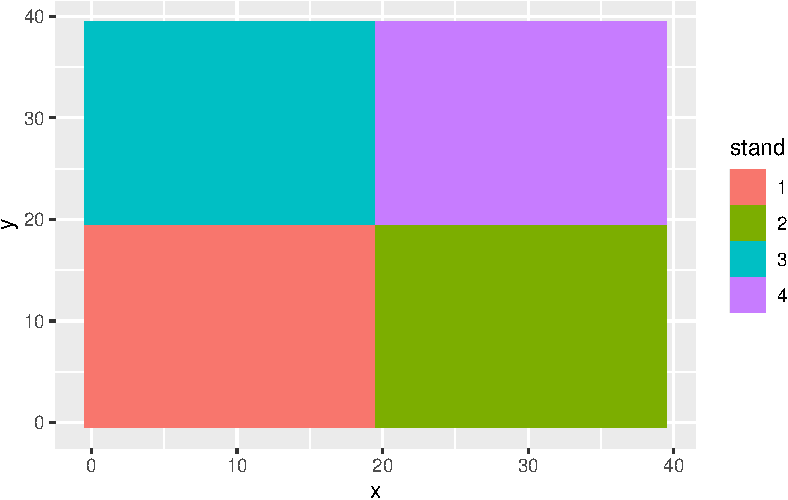
\includegraphics{Regression_estimator_files/figure-pdf/unnamed-chunk-1-1.pdf}

}

\end{figure}

\begin{Shaded}
\begin{Highlighting}[]
\FunctionTok{ggplot}\NormalTok{(example1,}\FunctionTok{aes}\NormalTok{(}\AttributeTok{x=}\NormalTok{x,}\AttributeTok{y=}\NormalTok{y,}\AttributeTok{fill=}\NormalTok{volume)) }\SpecialCharTok{+} \FunctionTok{geom\_tile}\NormalTok{()}
\end{Highlighting}
\end{Shaded}

\begin{figure}[H]

{\centering 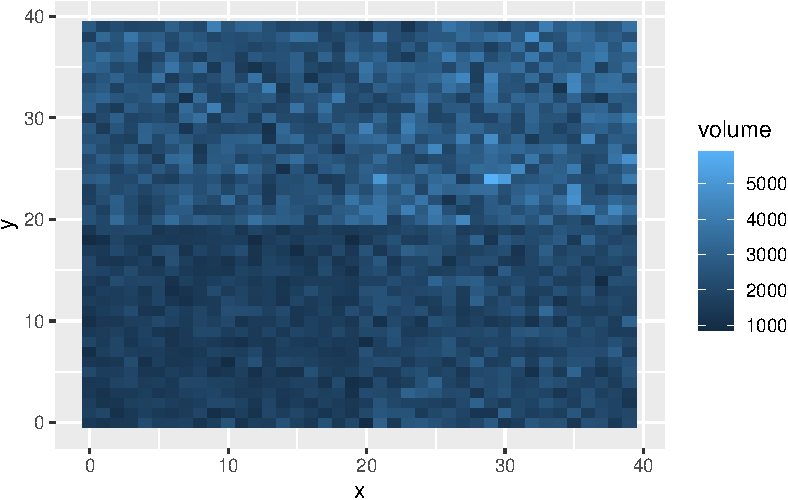
\includegraphics{Regression_estimator_files/figure-pdf/unnamed-chunk-1-2.pdf}

}

\end{figure}

\begin{Shaded}
\begin{Highlighting}[]
\FunctionTok{ggplot}\NormalTok{(example1,}\FunctionTok{aes}\NormalTok{(}\AttributeTok{x=}\NormalTok{x,}\AttributeTok{y=}\NormalTok{y,}\AttributeTok{fill=}\NormalTok{p95)) }\SpecialCharTok{+} \FunctionTok{geom\_tile}\NormalTok{()}
\end{Highlighting}
\end{Shaded}

\begin{figure}[H]

{\centering 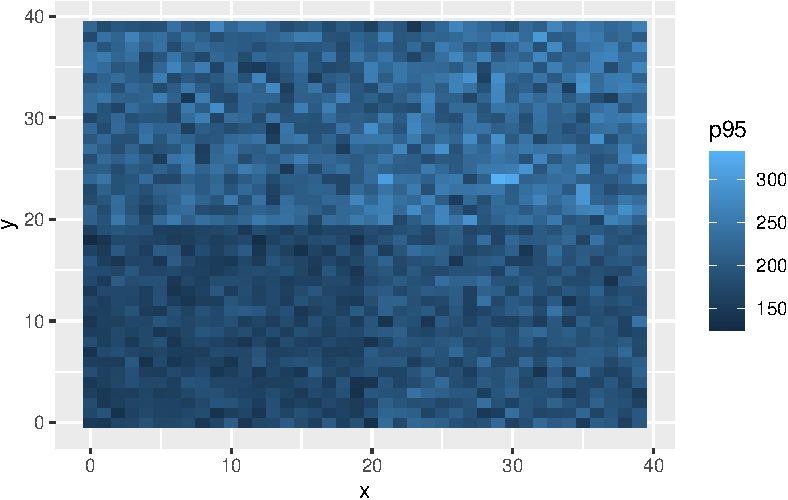
\includegraphics{Regression_estimator_files/figure-pdf/unnamed-chunk-1-3.pdf}

}

\end{figure}

\begin{Shaded}
\begin{Highlighting}[]
\NormalTok{example1}\SpecialCharTok{$}\NormalTok{volume }\OtherTok{\textless{}{-}} \FunctionTok{rnorm}\NormalTok{(}\DecValTok{1600}\NormalTok{,}\FloatTok{0.07}\SpecialCharTok{*}\NormalTok{example1}\SpecialCharTok{$}\NormalTok{p95}\FloatTok{+0.0005}\SpecialCharTok{*}\NormalTok{example1}\SpecialCharTok{$}\NormalTok{p95}\SpecialCharTok{\^{}}\DecValTok{2}\NormalTok{,}\FloatTok{0.008}\SpecialCharTok{*}\NormalTok{example1}\SpecialCharTok{$}\NormalTok{p95)}
\end{Highlighting}
\end{Shaded}

We will start estimating the average volume in the forest and in the
mean volume in each stand doing simple random sampling without
replacement. Having the volume of all grid units allows us to obtain the
true average volume in the forest.

\begin{Shaded}
\begin{Highlighting}[]
\NormalTok{true\_mean\_forest }\OtherTok{\textless{}{-}} \FunctionTok{mean}\NormalTok{(example1}\SpecialCharTok{$}\NormalTok{volume)}
\NormalTok{true\_mean\_stand1 }\OtherTok{\textless{}{-}} \FunctionTok{mean}\NormalTok{(example1}\SpecialCharTok{$}\NormalTok{volume[example1}\SpecialCharTok{$}\NormalTok{stand}\SpecialCharTok{==}\DecValTok{1}\NormalTok{])}
\NormalTok{true\_mean\_stand2 }\OtherTok{\textless{}{-}} \FunctionTok{mean}\NormalTok{(example1}\SpecialCharTok{$}\NormalTok{volume[example1}\SpecialCharTok{$}\NormalTok{stand}\SpecialCharTok{==}\DecValTok{2}\NormalTok{])}
\NormalTok{true\_mean\_stand3 }\OtherTok{\textless{}{-}} \FunctionTok{mean}\NormalTok{(example1}\SpecialCharTok{$}\NormalTok{volume[example1}\SpecialCharTok{$}\NormalTok{stand}\SpecialCharTok{==}\DecValTok{3}\NormalTok{])}
\NormalTok{true\_mean\_stand4 }\OtherTok{\textless{}{-}} \FunctionTok{mean}\NormalTok{(example1}\SpecialCharTok{$}\NormalTok{volume[example1}\SpecialCharTok{$}\NormalTok{stand}\SpecialCharTok{==}\DecValTok{4}\NormalTok{])}
\FunctionTok{print}\NormalTok{(}\StringTok{"True mean"}\NormalTok{)}
\end{Highlighting}
\end{Shaded}

\begin{verbatim}
[1] "True mean"
\end{verbatim}

\begin{Shaded}
\begin{Highlighting}[]
\NormalTok{true\_mean\_forest}
\end{Highlighting}
\end{Shaded}

\begin{verbatim}
[1] 34.3761
\end{verbatim}

\begin{Shaded}
\begin{Highlighting}[]
\FunctionTok{print}\NormalTok{(}\StringTok{"True mean stand 1"}\NormalTok{)}
\end{Highlighting}
\end{Shaded}

\begin{verbatim}
[1] "True mean stand 1"
\end{verbatim}

\begin{Shaded}
\begin{Highlighting}[]
\NormalTok{true\_mean\_stand1}
\end{Highlighting}
\end{Shaded}

\begin{verbatim}
[1] 26.21163
\end{verbatim}

\begin{Shaded}
\begin{Highlighting}[]
\FunctionTok{print}\NormalTok{(}\StringTok{"True mean stand 2"}\NormalTok{)}
\end{Highlighting}
\end{Shaded}

\begin{verbatim}
[1] "True mean stand 2"
\end{verbatim}

\begin{Shaded}
\begin{Highlighting}[]
\NormalTok{true\_mean\_stand2}
\end{Highlighting}
\end{Shaded}

\begin{verbatim}
[1] 31.74182
\end{verbatim}

\begin{Shaded}
\begin{Highlighting}[]
\FunctionTok{print}\NormalTok{(}\StringTok{"True mean stand 3"}\NormalTok{)}
\end{Highlighting}
\end{Shaded}

\begin{verbatim}
[1] "True mean stand 3"
\end{verbatim}

\begin{Shaded}
\begin{Highlighting}[]
\NormalTok{true\_mean\_stand3}
\end{Highlighting}
\end{Shaded}

\begin{verbatim}
[1] 37.01479
\end{verbatim}

\begin{Shaded}
\begin{Highlighting}[]
\FunctionTok{print}\NormalTok{(}\StringTok{"True mean stand 4"}\NormalTok{)}
\end{Highlighting}
\end{Shaded}

\begin{verbatim}
[1] "True mean stand 4"
\end{verbatim}

\begin{Shaded}
\begin{Highlighting}[]
\NormalTok{true\_mean\_stand4}
\end{Highlighting}
\end{Shaded}

\begin{verbatim}
[1] 42.53614
\end{verbatim}

\hypertarget{sample-mean-with-simple-random-sampling}{%
\subsection{Sample mean with simple random
sampling}\label{sample-mean-with-simple-random-sampling}}

Let's simulate our simple random sampling. We will repeat the simple
random sampling 100 with sample sizes of 16, 64, 96, 128, 160, 320 and
640 and plot our estimates to visualize the variance of doing simple
random sampling. We will store the result of each iteration in a
data.frame with our estimate, the sample size and the iteration.

\begin{Shaded}
\begin{Highlighting}[]
\NormalTok{repeats }\OtherTok{\textless{}{-}} \DecValTok{100}
\NormalTok{sample\_sizes }\OtherTok{\textless{}{-}} \FunctionTok{c}\NormalTok{(}\DecValTok{16}\NormalTok{, }\DecValTok{64}\NormalTok{, }\DecValTok{96}\NormalTok{, }\DecValTok{128}\NormalTok{, }\DecValTok{160}\NormalTok{, }\DecValTok{320}\NormalTok{, }\DecValTok{640}\NormalTok{ )}
\NormalTok{result }\OtherTok{\textless{}{-}} \FunctionTok{data.frame}\NormalTok{(}\AttributeTok{rep=}\FunctionTok{c}\NormalTok{(),}\AttributeTok{sample\_size=}\FunctionTok{c}\NormalTok{(),}
                      \AttributeTok{estimated\_mean\_forest=}\FunctionTok{c}\NormalTok{(),}
                      \AttributeTok{estimated\_mean\_stand1 =} \FunctionTok{c}\NormalTok{(),}
                      \AttributeTok{estimated\_mean\_stand2 =} \FunctionTok{c}\NormalTok{(),}
                      \AttributeTok{estimated\_mean\_stand3 =} \FunctionTok{c}\NormalTok{(),}
                      \AttributeTok{estimated\_mean\_stand4=}\FunctionTok{c}\NormalTok{())}
\NormalTok{cont }\OtherTok{\textless{}{-}} \DecValTok{1}
\ControlFlowTok{for}\NormalTok{(i }\ControlFlowTok{in} \DecValTok{1}\SpecialCharTok{:}\NormalTok{repeats)\{}
  \ControlFlowTok{for}\NormalTok{(j }\ControlFlowTok{in}\NormalTok{ sample\_sizes)\{}
    \CommentTok{\# get a sample of the indices of the data}
\NormalTok{    my\_sample}\OtherTok{\textless{}{-}} \FunctionTok{sample}\NormalTok{(}\FunctionTok{dim}\NormalTok{(example1)[}\DecValTok{1}\NormalTok{],j,}\AttributeTok{replace =} \ConstantTok{FALSE}\NormalTok{)}
    \CommentTok{\# subset the forest}
\NormalTok{    sampled\_data }\OtherTok{\textless{}{-}}\NormalTok{ example1[my\_sample,]}
    \CommentTok{\# store the rep and sample size}
\NormalTok{    result[cont,}\StringTok{"rep"}\NormalTok{]}\OtherTok{\textless{}{-}}\NormalTok{i}
\NormalTok{    result[cont,}\StringTok{"sample\_size"}\NormalTok{]}\OtherTok{\textless{}{-}}\NormalTok{j}
    \CommentTok{\# calculate the sample means for the forest and each stand}
\NormalTok{    result[cont,}\StringTok{"estimated\_mean\_forest"}\NormalTok{]}\OtherTok{\textless{}{-}}\FunctionTok{mean}\NormalTok{(sampled\_data}\SpecialCharTok{$}\NormalTok{volume)}
\NormalTok{    result[cont,}\StringTok{"estimated\_mean\_stand1"}\NormalTok{]}\OtherTok{\textless{}{-}}\FunctionTok{mean}\NormalTok{(sampled\_data}\SpecialCharTok{$}\NormalTok{volume[sampled\_data}\SpecialCharTok{$}\NormalTok{stand}\SpecialCharTok{==}\DecValTok{1}\NormalTok{])}
\NormalTok{    result[cont,}\StringTok{"estimated\_mean\_stand2"}\NormalTok{]}\OtherTok{\textless{}{-}}\FunctionTok{mean}\NormalTok{(sampled\_data}\SpecialCharTok{$}\NormalTok{volume[sampled\_data}\SpecialCharTok{$}\NormalTok{stand}\SpecialCharTok{==}\DecValTok{2}\NormalTok{])}
\NormalTok{    result[cont,}\StringTok{"estimated\_mean\_stand3"}\NormalTok{]}\OtherTok{\textless{}{-}}\FunctionTok{mean}\NormalTok{(sampled\_data}\SpecialCharTok{$}\NormalTok{volume[sampled\_data}\SpecialCharTok{$}\NormalTok{stand}\SpecialCharTok{==}\DecValTok{3}\NormalTok{])}
\NormalTok{    result[cont,}\StringTok{"estimated\_mean\_stand4"}\NormalTok{]}\OtherTok{\textless{}{-}}\FunctionTok{mean}\NormalTok{(sampled\_data}\SpecialCharTok{$}\NormalTok{volume[sampled\_data}\SpecialCharTok{$}\NormalTok{stand}\SpecialCharTok{==}\DecValTok{4}\NormalTok{])}
    \CommentTok{\# pass to next iteration}
\NormalTok{    cont }\OtherTok{\textless{}{-}}\NormalTok{ cont}\SpecialCharTok{+}\DecValTok{1}
\NormalTok{  \}}
\NormalTok{\}}
\CommentTok{\# Store the pre{-}calculated true values}
\NormalTok{result}\SpecialCharTok{$}\NormalTok{true\_mean\_forest}\OtherTok{\textless{}{-}}\NormalTok{true\_mean\_forest}
\NormalTok{result}\SpecialCharTok{$}\NormalTok{true\_mean\_stand1 }\OtherTok{\textless{}{-}}\NormalTok{ true\_mean\_stand1}
\NormalTok{result}\SpecialCharTok{$}\NormalTok{true\_mean\_stand2 }\OtherTok{\textless{}{-}}\NormalTok{ true\_mean\_stand2 }
\NormalTok{result}\SpecialCharTok{$}\NormalTok{true\_mean\_stand3 }\OtherTok{\textless{}{-}}\NormalTok{ true\_mean\_stand3 }
\NormalTok{result}\SpecialCharTok{$}\NormalTok{true\_mean\_stand4 }\OtherTok{\textless{}{-}}\NormalTok{ true\_mean\_stand4}
\end{Highlighting}
\end{Shaded}

Let's now plot our results as a function of the sample size. We will
simulate a precission requierement of +- 10\% in our estimates piloting
discontinuous lines around the true value

\begin{Shaded}
\begin{Highlighting}[]
\FunctionTok{plot}\NormalTok{(result}\SpecialCharTok{$}\NormalTok{sample\_size,result}\SpecialCharTok{$}\NormalTok{estimated\_mean\_forest,}\AttributeTok{ylim=}\FunctionTok{c}\NormalTok{(}\DecValTok{20}\NormalTok{,}\DecValTok{70}\NormalTok{),}
      \AttributeTok{main=}\StringTok{"Estimated means forest vs sample size"}\NormalTok{)}
\FunctionTok{abline}\NormalTok{(true\_mean\_forest,}\DecValTok{0}\NormalTok{,}\AttributeTok{col=}\StringTok{"blue"}\NormalTok{)}
\end{Highlighting}
\end{Shaded}

\begin{figure}[H]

{\centering 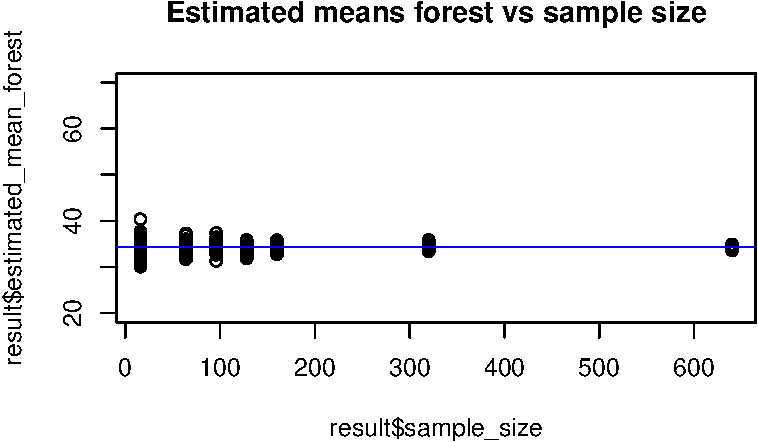
\includegraphics{Regression_estimator_files/figure-pdf/unnamed-chunk-4-1.pdf}

}

\end{figure}

\begin{Shaded}
\begin{Highlighting}[]
\FunctionTok{par}\NormalTok{(}\AttributeTok{mfrow=}\FunctionTok{c}\NormalTok{(}\DecValTok{2}\NormalTok{,}\DecValTok{2}\NormalTok{))}
\FunctionTok{plot}\NormalTok{(result}\SpecialCharTok{$}\NormalTok{sample\_size,result}\SpecialCharTok{$}\NormalTok{estimated\_mean\_stand1,}\AttributeTok{ylim=}\FunctionTok{c}\NormalTok{(}\DecValTok{20}\NormalTok{,}\DecValTok{70}\NormalTok{),}
      \AttributeTok{main=}\StringTok{"Estimated means stand 1 vs sample size"}\NormalTok{)}
\FunctionTok{abline}\NormalTok{(true\_mean\_stand1,}\DecValTok{0}\NormalTok{,}\AttributeTok{col=}\StringTok{"red"}\NormalTok{)}
\FunctionTok{plot}\NormalTok{(result}\SpecialCharTok{$}\NormalTok{sample\_size,result}\SpecialCharTok{$}\NormalTok{estimated\_mean\_stand2,}\AttributeTok{ylim=}\FunctionTok{c}\NormalTok{(}\DecValTok{20}\NormalTok{,}\DecValTok{70}\NormalTok{),}
      \AttributeTok{main=}\StringTok{"Estimated means stand 2 vs sample size"}\NormalTok{)}
\FunctionTok{abline}\NormalTok{(true\_mean\_stand2,}\DecValTok{0}\NormalTok{,}\AttributeTok{col=}\StringTok{"green"}\NormalTok{)}
\FunctionTok{plot}\NormalTok{(result}\SpecialCharTok{$}\NormalTok{sample\_size,result}\SpecialCharTok{$}\NormalTok{estimated\_mean\_stand3,}\AttributeTok{ylim=}\FunctionTok{c}\NormalTok{(}\DecValTok{20}\NormalTok{,}\DecValTok{70}\NormalTok{),}
      \AttributeTok{main=}\StringTok{"Estimated means stand 3 vs sample size"}\NormalTok{)}
\FunctionTok{abline}\NormalTok{(true\_mean\_stand3,}\DecValTok{0}\NormalTok{,}\AttributeTok{col=}\StringTok{"purple"}\NormalTok{)}
\FunctionTok{plot}\NormalTok{(result}\SpecialCharTok{$}\NormalTok{sample\_size,result}\SpecialCharTok{$}\NormalTok{estimated\_mean\_stand4,}\AttributeTok{ylim=}\FunctionTok{c}\NormalTok{(}\DecValTok{20}\NormalTok{,}\DecValTok{70}\NormalTok{),}
      \AttributeTok{main=}\StringTok{"Estimated means stand 4 vs sample size"}\NormalTok{)}
\FunctionTok{abline}\NormalTok{(true\_mean\_stand4,}\DecValTok{0}\NormalTok{,}\AttributeTok{col=}\StringTok{"orange"}\NormalTok{)}
\end{Highlighting}
\end{Shaded}

\begin{figure}[H]

{\centering 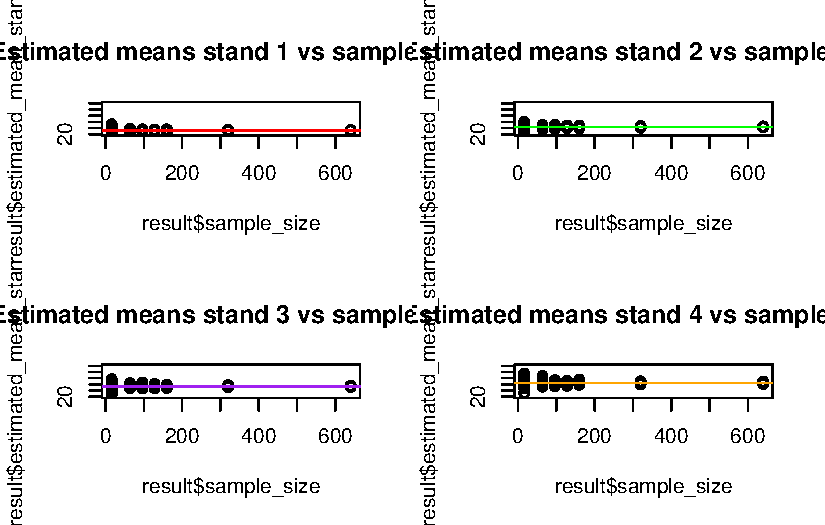
\includegraphics{Regression_estimator_files/figure-pdf/unnamed-chunk-4-2.pdf}

}

\end{figure}

\begin{Shaded}
\begin{Highlighting}[]
\FunctionTok{par}\NormalTok{(}\AttributeTok{mfrow=}\FunctionTok{c}\NormalTok{(}\DecValTok{1}\NormalTok{,}\DecValTok{2}\NormalTok{))}
\FunctionTok{plot}\NormalTok{(result}\SpecialCharTok{$}\NormalTok{sample\_size,result}\SpecialCharTok{$}\NormalTok{estimated\_mean\_forest,}\AttributeTok{ylim=}\FunctionTok{c}\NormalTok{(}\DecValTok{20}\NormalTok{,}\DecValTok{70}\NormalTok{),}
     \AttributeTok{main=}\StringTok{"Estimated means forest vs sample size"}\NormalTok{)}
\FunctionTok{abline}\NormalTok{(true\_mean\_forest,}\DecValTok{0}\NormalTok{,}\AttributeTok{col=}\StringTok{"blue"}\NormalTok{)}
\FunctionTok{plot}\NormalTok{(result}\SpecialCharTok{$}\NormalTok{sample\_size,result}\SpecialCharTok{$}\NormalTok{estimated\_mean\_stand4,}\AttributeTok{ylim=}\FunctionTok{c}\NormalTok{(}\DecValTok{20}\NormalTok{,}\DecValTok{70}\NormalTok{),}
      \AttributeTok{main=}\StringTok{"Estimated means stand 4 vs sample size"}\NormalTok{)}
\FunctionTok{abline}\NormalTok{(true\_mean\_stand4,}\DecValTok{0}\NormalTok{,}\AttributeTok{col=}\StringTok{"orange"}\NormalTok{)}
\end{Highlighting}
\end{Shaded}

\begin{figure}[H]

{\centering 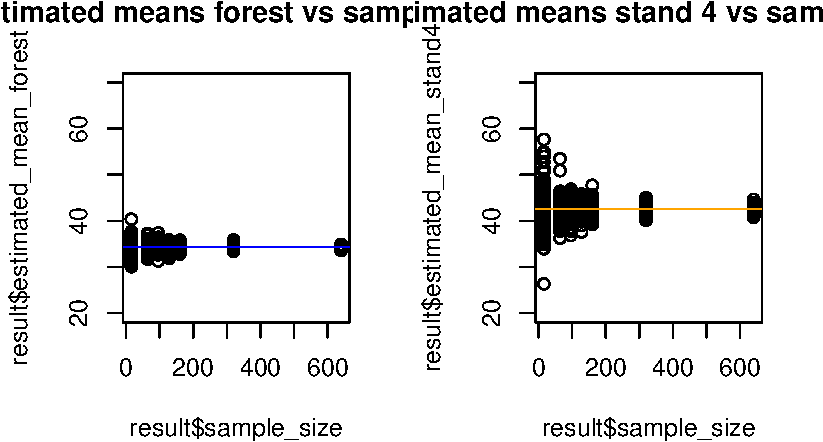
\includegraphics{Regression_estimator_files/figure-pdf/unnamed-chunk-4-3.pdf}

}

\end{figure}

Inspecting the generated figures we can observe the variance of our
estimates as a function of sample size and draw some interesting
conclusions.

\begin{enumerate}
\def\labelenumi{\arabic{enumi}.}
\item
  The variability of our estimates over repeated samples decreases with
  a pattern that resembles the graph of \(\sqrt{\frac{1}{n}}\)
\item
  As we know the sample mean is unbiased and, on average, tend to
  coincide with the true means for the forest and the stands.
\item
  When we compare the figure for the total forest and the figure for
  stand 4, we see that at some point, the sample size for stand 4
  becomes so small that the variability is very large.
\end{enumerate}

Now we are going to repeat the same process but instead of using the
sample mean we will use the auxiliary information to calculate the
regression estimator using p95 as auxiliary variable (X).

\begin{Shaded}
\begin{Highlighting}[]
\NormalTok{repeats }\OtherTok{\textless{}{-}} \DecValTok{100}
\NormalTok{sample\_sizes }\OtherTok{\textless{}{-}} \FunctionTok{c}\NormalTok{(}\DecValTok{16}\NormalTok{, }\DecValTok{64}\NormalTok{, }\DecValTok{96}\NormalTok{, }\DecValTok{128}\NormalTok{, }\DecValTok{160}\NormalTok{, }\DecValTok{320}\NormalTok{, }\DecValTok{640}\NormalTok{ )}
\NormalTok{result\_reg }\OtherTok{\textless{}{-}} \FunctionTok{data.frame}\NormalTok{(}\AttributeTok{rep=}\FunctionTok{c}\NormalTok{(),}\AttributeTok{sample\_size=}\FunctionTok{c}\NormalTok{(),}
                      \AttributeTok{estimated\_mean\_forest=}\FunctionTok{c}\NormalTok{(),}
                      \AttributeTok{estimated\_mean\_stand1 =} \FunctionTok{c}\NormalTok{(),}
                      \AttributeTok{estimated\_mean\_stand2 =} \FunctionTok{c}\NormalTok{(),}
                      \AttributeTok{estimated\_mean\_stand3 =} \FunctionTok{c}\NormalTok{(),}
                      \AttributeTok{estimated\_mean\_stand4=}\FunctionTok{c}\NormalTok{())}
\NormalTok{cont }\OtherTok{\textless{}{-}} \DecValTok{1}
\ControlFlowTok{for}\NormalTok{(i }\ControlFlowTok{in} \DecValTok{1}\SpecialCharTok{:}\NormalTok{repeats)\{}
  \ControlFlowTok{for}\NormalTok{(j }\ControlFlowTok{in}\NormalTok{ sample\_sizes)\{}
    \CommentTok{\# get a sample of the indices of the data}
\NormalTok{    my\_sample\_reg}\OtherTok{\textless{}{-}} \FunctionTok{sample}\NormalTok{(}\FunctionTok{dim}\NormalTok{(example1)[}\DecValTok{1}\NormalTok{],j,}\AttributeTok{replace =} \ConstantTok{FALSE}\NormalTok{)}
    \CommentTok{\# subset the forest and obtain the sample fit using OLS (lm function)}
\NormalTok{    sampled\_data\_reg }\OtherTok{\textless{}{-}}\NormalTok{ example1[my\_sample\_reg,]}
\NormalTok{    model\_forest }\OtherTok{\textless{}{-}} \FunctionTok{lm}\NormalTok{(volume}\SpecialCharTok{\textasciitilde{}}\NormalTok{p95,}\AttributeTok{data =}\NormalTok{ sampled\_data\_reg)}
\NormalTok{    media\_reg\_forest }\OtherTok{\textless{}{-}} \FunctionTok{mean}\NormalTok{(}\FunctionTok{predict}\NormalTok{(model\_forest,example1)) }\SpecialCharTok{+} \FunctionTok{mean}\NormalTok{(model\_forest}\SpecialCharTok{$}\NormalTok{residuals)}
    
    \CommentTok{\# now we will create subsamples for stands, obtain subsample fits for the stand and apply }
    \CommentTok{\# the regression estimator}
\NormalTok{    stand1 }\OtherTok{\textless{}{-}}\NormalTok{ sampled\_data\_reg[sampled\_data\_reg}\SpecialCharTok{$}\NormalTok{stand}\SpecialCharTok{==}\DecValTok{1}\NormalTok{,]}
\NormalTok{    media\_reg\_stand1 }\OtherTok{\textless{}{-}} \FunctionTok{try}\NormalTok{(\{}
\NormalTok{      model\_stand1 }\OtherTok{\textless{}{-}} \FunctionTok{lm}\NormalTok{(volume}\SpecialCharTok{\textasciitilde{}}\NormalTok{p95, }\AttributeTok{data=}\NormalTok{stand1)}
      \FunctionTok{mean}\NormalTok{(}\FunctionTok{predict}\NormalTok{(model\_stand1,example1[example1}\SpecialCharTok{$}\NormalTok{stand}\SpecialCharTok{==}\DecValTok{1}\NormalTok{,]))}\SpecialCharTok{+} \FunctionTok{mean}\NormalTok{(model\_stand1}\SpecialCharTok{$}\NormalTok{residuals)}
\NormalTok{    \})}
    \ControlFlowTok{if}\NormalTok{(}\FunctionTok{inherits}\NormalTok{(media\_reg\_stand1,}\StringTok{"try{-}error"}\NormalTok{))\{}
\NormalTok{      media\_reg\_stand1}\OtherTok{\textless{}{-}}\ConstantTok{NA}
\NormalTok{    \}}
    \CommentTok{\# repeat for stand 2}
\NormalTok{    stand2 }\OtherTok{\textless{}{-}}\NormalTok{ sampled\_data\_reg[sampled\_data\_reg}\SpecialCharTok{$}\NormalTok{stand}\SpecialCharTok{==}\DecValTok{2}\NormalTok{,]}
\NormalTok{    media\_reg\_stand2 }\OtherTok{\textless{}{-}} \FunctionTok{try}\NormalTok{(\{}
\NormalTok{      model\_stand2 }\OtherTok{\textless{}{-}} \FunctionTok{lm}\NormalTok{(volume}\SpecialCharTok{\textasciitilde{}}\NormalTok{p95, }\AttributeTok{data=}\NormalTok{stand2)}
      \FunctionTok{mean}\NormalTok{(}\FunctionTok{predict}\NormalTok{(model\_stand2,example1[example1}\SpecialCharTok{$}\NormalTok{stand}\SpecialCharTok{==}\DecValTok{2}\NormalTok{,])) }\SpecialCharTok{+} \FunctionTok{mean}\NormalTok{(model\_stand2}\SpecialCharTok{$}\NormalTok{residuals)}
\NormalTok{    \})}
    \CommentTok{\# bypass very low stand sample size}
    \ControlFlowTok{if}\NormalTok{(}\FunctionTok{inherits}\NormalTok{(media\_reg\_stand2,}\StringTok{"try{-}error"}\NormalTok{))\{}
\NormalTok{      media\_reg\_stand2}\OtherTok{\textless{}{-}}\ConstantTok{NA}
\NormalTok{    \}}
    \CommentTok{\# repeat for stand 3}
\NormalTok{    stand3 }\OtherTok{\textless{}{-}}\NormalTok{ sampled\_data\_reg[sampled\_data\_reg}\SpecialCharTok{$}\NormalTok{stand}\SpecialCharTok{==}\DecValTok{3}\NormalTok{,]}
\NormalTok{    media\_reg\_stand3 }\OtherTok{\textless{}{-}} \FunctionTok{try}\NormalTok{(\{}
\NormalTok{      model\_stand3 }\OtherTok{\textless{}{-}} \FunctionTok{lm}\NormalTok{(volume}\SpecialCharTok{\textasciitilde{}}\NormalTok{p95, }\AttributeTok{data=}\NormalTok{stand3)}
      \FunctionTok{mean}\NormalTok{(}\FunctionTok{predict}\NormalTok{(model\_stand3,example1[example1}\SpecialCharTok{$}\NormalTok{stand}\SpecialCharTok{==}\DecValTok{3}\NormalTok{,])) }\SpecialCharTok{+} \FunctionTok{mean}\NormalTok{(model\_stand3}\SpecialCharTok{$}\NormalTok{residuals)}
\NormalTok{    \})}
    \CommentTok{\# bypass very low stand sample size}
    \ControlFlowTok{if}\NormalTok{(}\FunctionTok{inherits}\NormalTok{(media\_reg\_stand3,}\StringTok{"try{-}error"}\NormalTok{))\{}
\NormalTok{      media\_reg\_stand3}\OtherTok{\textless{}{-}}\ConstantTok{NA}
\NormalTok{    \}}
    
    \CommentTok{\# repeat for stand 4}
\NormalTok{    stand4 }\OtherTok{\textless{}{-}}\NormalTok{ sampled\_data\_reg[sampled\_data\_reg}\SpecialCharTok{$}\NormalTok{stand}\SpecialCharTok{==}\DecValTok{4}\NormalTok{,]}
\NormalTok{    media\_reg\_stand4 }\OtherTok{\textless{}{-}} \FunctionTok{try}\NormalTok{(\{}
\NormalTok{      model\_stand4 }\OtherTok{\textless{}{-}} \FunctionTok{lm}\NormalTok{(volume}\SpecialCharTok{\textasciitilde{}}\NormalTok{p95, }\AttributeTok{data=}\NormalTok{stand4)}
      \FunctionTok{mean}\NormalTok{(}\FunctionTok{predict}\NormalTok{(model\_stand4,example1[example1}\SpecialCharTok{$}\NormalTok{stand}\SpecialCharTok{==}\DecValTok{4}\NormalTok{,])) }\SpecialCharTok{+} \FunctionTok{mean}\NormalTok{(model\_stand4}\SpecialCharTok{$}\NormalTok{residuals)}
\NormalTok{    \})}
    \CommentTok{\# bypass very low stand sample size}
    \ControlFlowTok{if}\NormalTok{(}\FunctionTok{inherits}\NormalTok{(media\_reg\_stand4,}\StringTok{"try{-}error"}\NormalTok{))\{}
\NormalTok{      media\_reg\_stand4}\OtherTok{\textless{}{-}}\ConstantTok{NA}
\NormalTok{    \}}
    
    
    
\NormalTok{    stand2 }\OtherTok{\textless{}{-}}\NormalTok{ sampled\_data\_reg[sampled\_data\_reg}\SpecialCharTok{$}\NormalTok{stand}\SpecialCharTok{==}\DecValTok{2}\NormalTok{,]}
\NormalTok{    stand3 }\OtherTok{\textless{}{-}}\NormalTok{ sampled\_data\_reg[sampled\_data\_reg}\SpecialCharTok{$}\NormalTok{stand}\SpecialCharTok{==}\DecValTok{3}\NormalTok{,]}
\NormalTok{    stand4 }\OtherTok{\textless{}{-}}\NormalTok{ sampled\_data\_reg[sampled\_data\_reg}\SpecialCharTok{$}\NormalTok{stand}\SpecialCharTok{==}\DecValTok{4}\NormalTok{,]}
    \CommentTok{\# store the rep and sample size}
\NormalTok{    result\_reg[cont,}\StringTok{"rep"}\NormalTok{]}\OtherTok{\textless{}{-}}\NormalTok{i}
\NormalTok{    result\_reg[cont,}\StringTok{"sample\_size"}\NormalTok{]}\OtherTok{\textless{}{-}}\NormalTok{j}
    \CommentTok{\# calculate the sample means for the forest and each stand}
\NormalTok{    result\_reg[cont,}\StringTok{"estimated\_mean\_forest"}\NormalTok{]}\OtherTok{\textless{}{-}}\NormalTok{media\_reg\_forest}
\NormalTok{    result\_reg[cont,}\StringTok{"estimated\_mean\_stand1"}\NormalTok{]}\OtherTok{\textless{}{-}}\NormalTok{media\_reg\_stand1}
\NormalTok{    result\_reg[cont,}\StringTok{"estimated\_mean\_stand2"}\NormalTok{]}\OtherTok{\textless{}{-}}\NormalTok{media\_reg\_stand2}
\NormalTok{    result\_reg[cont,}\StringTok{"estimated\_mean\_stand3"}\NormalTok{]}\OtherTok{\textless{}{-}}\NormalTok{media\_reg\_stand3}
\NormalTok{    result\_reg[cont,}\StringTok{"estimated\_mean\_stand4"}\NormalTok{]}\OtherTok{\textless{}{-}}\NormalTok{media\_reg\_stand4}
    \CommentTok{\# pass to next iteration}
\NormalTok{    cont }\OtherTok{\textless{}{-}}\NormalTok{ cont}\SpecialCharTok{+}\DecValTok{1}
\NormalTok{  \}}
\NormalTok{\}}
\end{Highlighting}
\end{Shaded}

\begin{verbatim}
Warning in predict.lm(model_stand3, example1[example1$stand == 3, ]):
prediction from rank-deficient fit; attr(*, "non-estim") has doubtful cases
\end{verbatim}

\begin{verbatim}
Warning in predict.lm(model_stand1, example1[example1$stand == 1, ]):
prediction from rank-deficient fit; attr(*, "non-estim") has doubtful cases
\end{verbatim}

\begin{verbatim}
Warning in predict.lm(model_stand4, example1[example1$stand == 4, ]):
prediction from rank-deficient fit; attr(*, "non-estim") has doubtful cases
\end{verbatim}

\begin{verbatim}
Warning in predict.lm(model_stand1, example1[example1$stand == 1, ]):
prediction from rank-deficient fit; attr(*, "non-estim") has doubtful cases
\end{verbatim}

\begin{verbatim}
Error in lm.fit(x, y, offset = offset, singular.ok = singular.ok, ...) : 
  0 (non-NA) cases
\end{verbatim}

\begin{verbatim}
Warning in predict.lm(model_stand2, example1[example1$stand == 2, ]):
prediction from rank-deficient fit; attr(*, "non-estim") has doubtful cases
\end{verbatim}

\begin{verbatim}
Warning in predict.lm(model_stand3, example1[example1$stand == 3, ]):
prediction from rank-deficient fit; attr(*, "non-estim") has doubtful cases
\end{verbatim}

\begin{verbatim}
Warning in predict.lm(model_stand1, example1[example1$stand == 1, ]):
prediction from rank-deficient fit; attr(*, "non-estim") has doubtful cases
Warning in predict.lm(model_stand1, example1[example1$stand == 1, ]):
prediction from rank-deficient fit; attr(*, "non-estim") has doubtful cases
Warning in predict.lm(model_stand1, example1[example1$stand == 1, ]):
prediction from rank-deficient fit; attr(*, "non-estim") has doubtful cases
Warning in predict.lm(model_stand1, example1[example1$stand == 1, ]):
prediction from rank-deficient fit; attr(*, "non-estim") has doubtful cases
\end{verbatim}

\begin{verbatim}
Warning in predict.lm(model_stand3, example1[example1$stand == 3, ]):
prediction from rank-deficient fit; attr(*, "non-estim") has doubtful cases
\end{verbatim}

\begin{verbatim}
Warning in predict.lm(model_stand1, example1[example1$stand == 1, ]):
prediction from rank-deficient fit; attr(*, "non-estim") has doubtful cases
\end{verbatim}

\begin{verbatim}
Warning in predict.lm(model_stand4, example1[example1$stand == 4, ]):
prediction from rank-deficient fit; attr(*, "non-estim") has doubtful cases
\end{verbatim}

\begin{verbatim}
Warning in predict.lm(model_stand3, example1[example1$stand == 3, ]):
prediction from rank-deficient fit; attr(*, "non-estim") has doubtful cases
\end{verbatim}

\begin{verbatim}
Warning in predict.lm(model_stand4, example1[example1$stand == 4, ]):
prediction from rank-deficient fit; attr(*, "non-estim") has doubtful cases
\end{verbatim}

\begin{verbatim}
Error in lm.fit(x, y, offset = offset, singular.ok = singular.ok, ...) : 
  0 (non-NA) cases
\end{verbatim}

\begin{verbatim}
Warning in predict.lm(model_stand1, example1[example1$stand == 1, ]):
prediction from rank-deficient fit; attr(*, "non-estim") has doubtful cases
Warning in predict.lm(model_stand1, example1[example1$stand == 1, ]):
prediction from rank-deficient fit; attr(*, "non-estim") has doubtful cases
Warning in predict.lm(model_stand1, example1[example1$stand == 1, ]):
prediction from rank-deficient fit; attr(*, "non-estim") has doubtful cases
Warning in predict.lm(model_stand1, example1[example1$stand == 1, ]):
prediction from rank-deficient fit; attr(*, "non-estim") has doubtful cases
\end{verbatim}

\begin{verbatim}
Warning in predict.lm(model_stand2, example1[example1$stand == 2, ]):
prediction from rank-deficient fit; attr(*, "non-estim") has doubtful cases
\end{verbatim}

\begin{verbatim}
Warning in predict.lm(model_stand3, example1[example1$stand == 3, ]):
prediction from rank-deficient fit; attr(*, "non-estim") has doubtful cases
\end{verbatim}

\begin{verbatim}
Warning in predict.lm(model_stand4, example1[example1$stand == 4, ]):
prediction from rank-deficient fit; attr(*, "non-estim") has doubtful cases
\end{verbatim}

\begin{verbatim}
Warning in predict.lm(model_stand3, example1[example1$stand == 3, ]):
prediction from rank-deficient fit; attr(*, "non-estim") has doubtful cases
\end{verbatim}

\begin{verbatim}
Warning in predict.lm(model_stand2, example1[example1$stand == 2, ]):
prediction from rank-deficient fit; attr(*, "non-estim") has doubtful cases
\end{verbatim}

\begin{verbatim}
Warning in predict.lm(model_stand3, example1[example1$stand == 3, ]):
prediction from rank-deficient fit; attr(*, "non-estim") has doubtful cases
Warning in predict.lm(model_stand3, example1[example1$stand == 3, ]):
prediction from rank-deficient fit; attr(*, "non-estim") has doubtful cases
Warning in predict.lm(model_stand3, example1[example1$stand == 3, ]):
prediction from rank-deficient fit; attr(*, "non-estim") has doubtful cases
\end{verbatim}

\begin{Shaded}
\begin{Highlighting}[]
\CommentTok{\# Store the pre{-}calculated true values}
\NormalTok{result\_reg}\SpecialCharTok{$}\NormalTok{true\_mean\_forest}\OtherTok{\textless{}{-}}\NormalTok{true\_mean\_forest}
\NormalTok{result\_reg}\SpecialCharTok{$}\NormalTok{true\_mean\_stand1 }\OtherTok{\textless{}{-}}\NormalTok{ true\_mean\_stand1}
\NormalTok{result\_reg}\SpecialCharTok{$}\NormalTok{true\_mean\_stand2 }\OtherTok{\textless{}{-}}\NormalTok{ true\_mean\_stand2 }
\NormalTok{result\_reg}\SpecialCharTok{$}\NormalTok{true\_mean\_stand3 }\OtherTok{\textless{}{-}}\NormalTok{ true\_mean\_stand3 }
\NormalTok{result\_reg}\SpecialCharTok{$}\NormalTok{true\_mean\_stand4 }\OtherTok{\textless{}{-}}\NormalTok{ true\_mean\_stand4}
\end{Highlighting}
\end{Shaded}

No let's plot the results

\begin{Shaded}
\begin{Highlighting}[]
\FunctionTok{plot}\NormalTok{(result\_reg}\SpecialCharTok{$}\NormalTok{sample\_size,result\_reg}\SpecialCharTok{$}\NormalTok{estimated\_mean\_forest,}\AttributeTok{ylim=}\FunctionTok{c}\NormalTok{(}\DecValTok{20}\NormalTok{,}\DecValTok{70}\NormalTok{),}
      \AttributeTok{main=}\StringTok{"Estimated means forest vs sample size"}\NormalTok{)}
\FunctionTok{abline}\NormalTok{(true\_mean\_forest,}\DecValTok{0}\NormalTok{,}\AttributeTok{col=}\StringTok{"blue"}\NormalTok{)}
\end{Highlighting}
\end{Shaded}

\begin{figure}[H]

{\centering 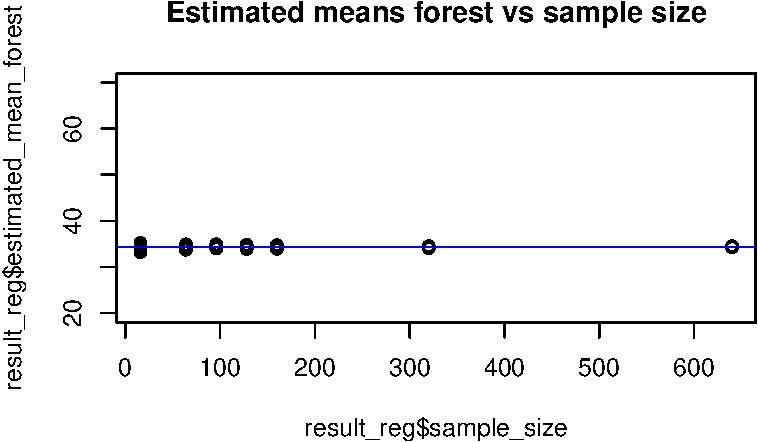
\includegraphics{Regression_estimator_files/figure-pdf/unnamed-chunk-6-1.pdf}

}

\end{figure}

\begin{Shaded}
\begin{Highlighting}[]
\FunctionTok{par}\NormalTok{(}\AttributeTok{mfrow=}\FunctionTok{c}\NormalTok{(}\DecValTok{2}\NormalTok{,}\DecValTok{2}\NormalTok{))}
\FunctionTok{plot}\NormalTok{(result\_reg}\SpecialCharTok{$}\NormalTok{sample\_size,result\_reg}\SpecialCharTok{$}\NormalTok{estimated\_mean\_stand1,}\AttributeTok{ylim=}\FunctionTok{c}\NormalTok{(}\DecValTok{20}\NormalTok{,}\DecValTok{70}\NormalTok{),}
      \AttributeTok{main=}\StringTok{"Estimated means stand 1 vs sample size"}\NormalTok{)}
\FunctionTok{abline}\NormalTok{(true\_mean\_stand1,}\DecValTok{0}\NormalTok{,}\AttributeTok{col=}\StringTok{"red"}\NormalTok{)}
\FunctionTok{plot}\NormalTok{(result\_reg}\SpecialCharTok{$}\NormalTok{sample\_size,result\_reg}\SpecialCharTok{$}\NormalTok{estimated\_mean\_stand2,}\AttributeTok{ylim=}\FunctionTok{c}\NormalTok{(}\DecValTok{20}\NormalTok{,}\DecValTok{70}\NormalTok{),}
      \AttributeTok{main=}\StringTok{"Estimated means stand 2 vs sample size"}\NormalTok{)}
\FunctionTok{abline}\NormalTok{(true\_mean\_stand2,}\DecValTok{0}\NormalTok{,}\AttributeTok{col=}\StringTok{"green"}\NormalTok{)}
\FunctionTok{plot}\NormalTok{(result\_reg}\SpecialCharTok{$}\NormalTok{sample\_size,result\_reg}\SpecialCharTok{$}\NormalTok{estimated\_mean\_stand3,}\AttributeTok{ylim=}\FunctionTok{c}\NormalTok{(}\DecValTok{20}\NormalTok{,}\DecValTok{70}\NormalTok{),}
      \AttributeTok{main=}\StringTok{"Estimated means stand 3 vs sample size"}\NormalTok{)}
\FunctionTok{abline}\NormalTok{(true\_mean\_stand3,}\DecValTok{0}\NormalTok{,}\AttributeTok{col=}\StringTok{"purple"}\NormalTok{)}
\FunctionTok{plot}\NormalTok{(result\_reg}\SpecialCharTok{$}\NormalTok{sample\_size,result\_reg}\SpecialCharTok{$}\NormalTok{estimated\_mean\_stand4,}\AttributeTok{ylim=}\FunctionTok{c}\NormalTok{(}\DecValTok{20}\NormalTok{,}\DecValTok{70}\NormalTok{),}
      \AttributeTok{main=}\StringTok{"Estimated means stand 4 vs sample size"}\NormalTok{)}
\FunctionTok{abline}\NormalTok{(true\_mean\_stand4,}\DecValTok{0}\NormalTok{,}\AttributeTok{col=}\StringTok{"orange"}\NormalTok{)}
\end{Highlighting}
\end{Shaded}

\begin{figure}[H]

{\centering 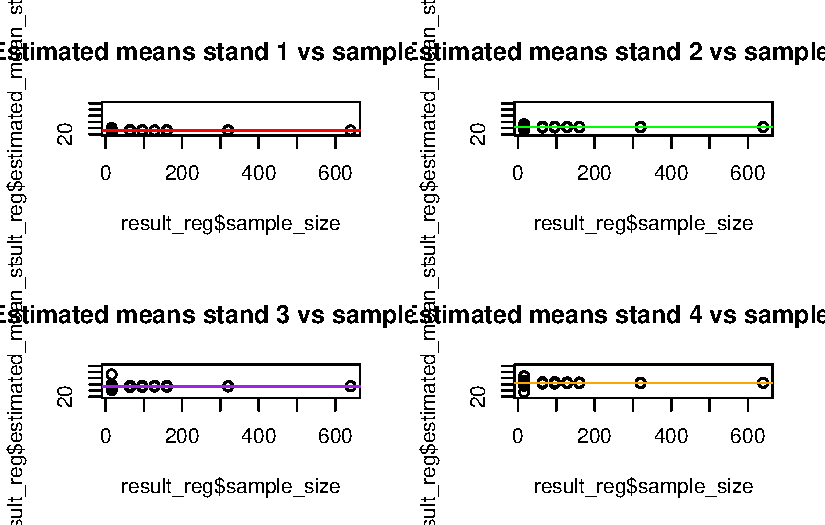
\includegraphics{Regression_estimator_files/figure-pdf/unnamed-chunk-6-2.pdf}

}

\end{figure}

\begin{Shaded}
\begin{Highlighting}[]
\FunctionTok{par}\NormalTok{(}\AttributeTok{mfrow=}\FunctionTok{c}\NormalTok{(}\DecValTok{1}\NormalTok{,}\DecValTok{2}\NormalTok{))}
\FunctionTok{plot}\NormalTok{(result\_reg}\SpecialCharTok{$}\NormalTok{sample\_size,result\_reg}\SpecialCharTok{$}\NormalTok{estimated\_mean\_forest,}\AttributeTok{ylim=}\FunctionTok{c}\NormalTok{(}\DecValTok{20}\NormalTok{,}\DecValTok{70}\NormalTok{),}
     \AttributeTok{main=}\StringTok{"Estimated means forest vs sample size"}\NormalTok{)}
\FunctionTok{abline}\NormalTok{(true\_mean\_forest,}\DecValTok{0}\NormalTok{,}\AttributeTok{col=}\StringTok{"blue"}\NormalTok{)}
\FunctionTok{plot}\NormalTok{(result\_reg}\SpecialCharTok{$}\NormalTok{sample\_size,result\_reg}\SpecialCharTok{$}\NormalTok{estimated\_mean\_stand4,}\AttributeTok{ylim=}\FunctionTok{c}\NormalTok{(}\DecValTok{20}\NormalTok{,}\DecValTok{70}\NormalTok{),}
      \AttributeTok{main=}\StringTok{"Estimated means stand 4 vs sample size"}\NormalTok{)}
\FunctionTok{abline}\NormalTok{(true\_mean\_stand4,}\DecValTok{0}\NormalTok{,}\AttributeTok{col=}\StringTok{"orange"}\NormalTok{)}
\end{Highlighting}
\end{Shaded}

\begin{figure}[H]

{\centering 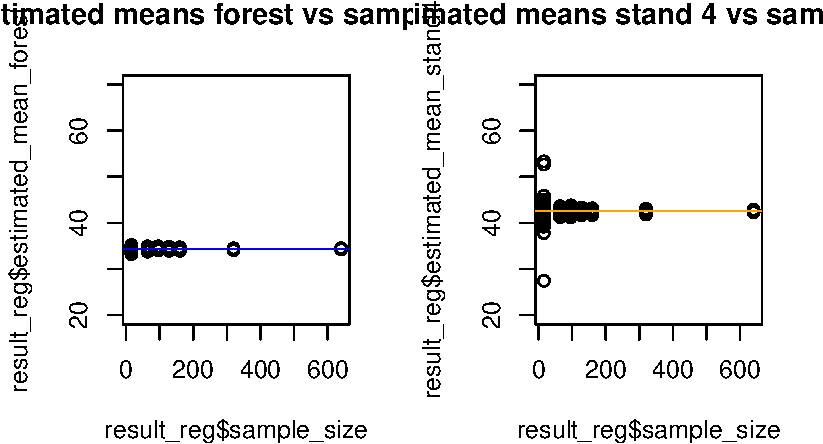
\includegraphics{Regression_estimator_files/figure-pdf/unnamed-chunk-6-3.pdf}

}

\end{figure}

If we observe the plots for the regression estimator we can see:

\begin{itemize}
\item
  The pattern with \(\sqrt{\frac{1}{n}}\) is also there, but this time
  the variability is smaller.
\item
  For all sample sizes, the estimates over repeated samples concentrate
  around the true values.
\item
  As before, the estimates for the entire forest have much lower
  variability than estimates for single stands.
\item
  You probably obtained some warnings in the process becasue some stands
  were never sampled or had very small sampled sizes.
\end{itemize}

\hypertarget{regression-estimator-with-simple-random-sampling}{%
\subsection{Regression estimator with simple random
sampling}\label{regression-estimator-with-simple-random-sampling}}

Let's now compare use the regression estimator. We will simulate a
precision requirement of +- 10\% in our estimates plotting discontinuous
lines around the true value

\begin{Shaded}
\begin{Highlighting}[]
\FunctionTok{par}\NormalTok{(}\AttributeTok{mfrow=}\FunctionTok{c}\NormalTok{(}\DecValTok{2}\NormalTok{,}\DecValTok{2}\NormalTok{))}
\FunctionTok{plot}\NormalTok{(result\_reg}\SpecialCharTok{$}\NormalTok{sample\_size,result\_reg}\SpecialCharTok{$}\NormalTok{estimated\_mean\_forest,}\AttributeTok{ylim=}\FunctionTok{c}\NormalTok{(}\DecValTok{20}\NormalTok{,}\DecValTok{70}\NormalTok{),}
     \AttributeTok{main=}\StringTok{"Regression estimator"}\NormalTok{)}
\FunctionTok{abline}\NormalTok{(true\_mean\_forest,}\DecValTok{0}\NormalTok{,}\AttributeTok{col=}\StringTok{"blue"}\NormalTok{)}
\FunctionTok{abline}\NormalTok{(true\_mean\_forest}\FloatTok{+0.1}\SpecialCharTok{*}\NormalTok{true\_mean\_forest,}\DecValTok{0}\NormalTok{,}\AttributeTok{col=}\StringTok{"blue"}\NormalTok{,}\AttributeTok{lty=}\DecValTok{2}\NormalTok{)}
\FunctionTok{abline}\NormalTok{(true\_mean\_forest}\FloatTok{{-}0.1}\SpecialCharTok{*}\NormalTok{true\_mean\_forest,}\DecValTok{0}\NormalTok{,}\AttributeTok{col=}\StringTok{"blue"}\NormalTok{,}\AttributeTok{lty=}\DecValTok{2}\NormalTok{)}
\FunctionTok{plot}\NormalTok{(result}\SpecialCharTok{$}\NormalTok{sample\_size,result}\SpecialCharTok{$}\NormalTok{estimated\_mean\_forest,}\AttributeTok{ylim=}\FunctionTok{c}\NormalTok{(}\DecValTok{20}\NormalTok{,}\DecValTok{70}\NormalTok{),}
     \AttributeTok{main=}\StringTok{"Sample mean"}\NormalTok{)}
\FunctionTok{abline}\NormalTok{(true\_mean\_forest}\FloatTok{+0.1}\SpecialCharTok{*}\NormalTok{true\_mean\_forest,}\DecValTok{0}\NormalTok{,}\AttributeTok{col=}\StringTok{"blue"}\NormalTok{,}\AttributeTok{lty=}\DecValTok{2}\NormalTok{)}
\FunctionTok{abline}\NormalTok{(true\_mean\_forest}\FloatTok{{-}0.1}\SpecialCharTok{*}\NormalTok{true\_mean\_forest,}\DecValTok{0}\NormalTok{,}\AttributeTok{col=}\StringTok{"blue"}\NormalTok{,}\AttributeTok{lty=}\DecValTok{2}\NormalTok{)}


\FunctionTok{plot}\NormalTok{(result\_reg}\SpecialCharTok{$}\NormalTok{sample\_size,result\_reg}\SpecialCharTok{$}\NormalTok{estimated\_mean\_stand4,}\AttributeTok{ylim=}\FunctionTok{c}\NormalTok{(}\DecValTok{20}\NormalTok{,}\DecValTok{70}\NormalTok{),}
      \AttributeTok{main=}\StringTok{"Regression estimator"}\NormalTok{)}
\FunctionTok{abline}\NormalTok{(true\_mean\_stand4,}\DecValTok{0}\NormalTok{,}\AttributeTok{col=}\StringTok{"orange"}\NormalTok{)}
\FunctionTok{abline}\NormalTok{(true\_mean\_stand4}\FloatTok{+0.1}\SpecialCharTok{*}\NormalTok{true\_mean\_stand4,}\DecValTok{0}\NormalTok{,}\AttributeTok{col=}\StringTok{"orange"}\NormalTok{,}\AttributeTok{lty=}\DecValTok{2}\NormalTok{)}
\FunctionTok{abline}\NormalTok{(true\_mean\_stand4}\FloatTok{{-}0.1}\SpecialCharTok{*}\NormalTok{true\_mean\_stand4,}\DecValTok{0}\NormalTok{,}\AttributeTok{col=}\StringTok{"orange"}\NormalTok{,}\AttributeTok{lty=}\DecValTok{2}\NormalTok{)}
\FunctionTok{plot}\NormalTok{(result\_reg}\SpecialCharTok{$}\NormalTok{sample\_size,result\_reg}\SpecialCharTok{$}\NormalTok{estimated\_mean\_stand4,}\AttributeTok{ylim=}\FunctionTok{c}\NormalTok{(}\DecValTok{20}\NormalTok{,}\DecValTok{70}\NormalTok{),}
      \AttributeTok{main=}\StringTok{"Sample mean"}\NormalTok{)}
\FunctionTok{abline}\NormalTok{(true\_mean\_stand4,}\DecValTok{0}\NormalTok{,}\AttributeTok{col=}\StringTok{"orange"}\NormalTok{)}
\FunctionTok{abline}\NormalTok{(true\_mean\_stand4}\FloatTok{+0.1}\SpecialCharTok{*}\NormalTok{true\_mean\_stand4,}\DecValTok{0}\NormalTok{,}\AttributeTok{col=}\StringTok{"orange"}\NormalTok{,}\AttributeTok{lty=}\DecValTok{2}\NormalTok{)}
\FunctionTok{abline}\NormalTok{(true\_mean\_stand4}\FloatTok{{-}0.1}\SpecialCharTok{*}\NormalTok{true\_mean\_stand4,}\DecValTok{0}\NormalTok{,}\AttributeTok{col=}\StringTok{"orange"}\NormalTok{,}\AttributeTok{lty=}\DecValTok{2}\NormalTok{)}
\end{Highlighting}
\end{Shaded}

\begin{figure}[H]

{\centering 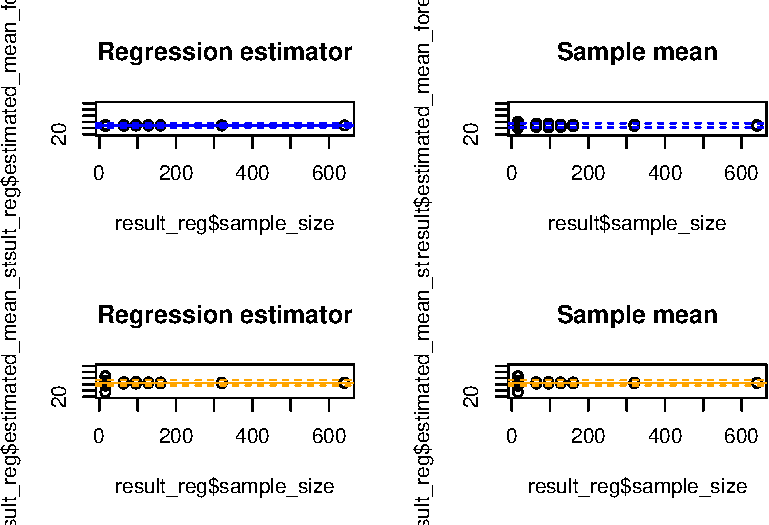
\includegraphics{Regression_estimator_files/figure-pdf/unnamed-chunk-7-1.pdf}

}

\end{figure}

When comparing the sample mean to the regression estimator, we can
observe that:

\begin{itemize}
\item
  For the entire forest the regression estimator does much better for
  all sample sizes. This is because the relationship between volume and
  p95 can be approximated well by a linear function. The relationship,
  however, is not linear, it was created with the code spinet below, but
  this method does not rely on assuming that a linear relationship
  exists.
\item
  For both methods variability for stands was larger and for small
  sample sizes variances were large.
\end{itemize}

\ul{\textbf{This is the small area estimation problem. We have reach to
a point where even using auxiliary information with a large correlation
with our response variable does not allow us to obtain reliable
estimates.}}

\begin{Shaded}
\begin{Highlighting}[]
\NormalTok{id }\OtherTok{\textless{}{-}} \DecValTok{1}\SpecialCharTok{:}\DecValTok{1600}
\NormalTok{x }\OtherTok{\textless{}{-}} \FunctionTok{rep}\NormalTok{(}\DecValTok{0}\SpecialCharTok{:}\DecValTok{39}\NormalTok{,}\AttributeTok{each=}\DecValTok{40}\NormalTok{)}
\NormalTok{y }\OtherTok{\textless{}{-}} \FunctionTok{rep}\NormalTok{(}\DecValTok{0}\SpecialCharTok{:}\DecValTok{39}\NormalTok{,}\AttributeTok{times=}\DecValTok{40}\NormalTok{)}
\NormalTok{stand }\OtherTok{\textless{}{-}}\NormalTok{ (}\DecValTok{1}\SpecialCharTok{+}\NormalTok{x}\SpecialCharTok{\%/\%}\DecValTok{20}\NormalTok{) }\SpecialCharTok{+}\DecValTok{2}\SpecialCharTok{*}\NormalTok{(y}\SpecialCharTok{\%/\%}\DecValTok{20}\NormalTok{)}
\NormalTok{p95 }\OtherTok{\textless{}{-}} \FunctionTok{rnorm}\NormalTok{(}\DecValTok{1600}\NormalTok{,}\DecValTok{150}\SpecialCharTok{+}\DecValTok{20}\SpecialCharTok{*}\NormalTok{stand,}\DecValTok{10}\SpecialCharTok{+}\DecValTok{5}\SpecialCharTok{*}\NormalTok{stand)}
\NormalTok{volume }\OtherTok{\textless{}{-}} \FunctionTok{rnorm}\NormalTok{(}\DecValTok{1600}\NormalTok{,p95}\FloatTok{+0.05}\SpecialCharTok{*}\NormalTok{p95}\SpecialCharTok{\^{}}\DecValTok{2}\NormalTok{,}\DecValTok{100}\NormalTok{)}
\NormalTok{example1 }\OtherTok{\textless{}{-}} \FunctionTok{data.frame}\NormalTok{(}\AttributeTok{id=}\NormalTok{id,}\AttributeTok{x=}\NormalTok{x,}\AttributeTok{y=}\NormalTok{y,}\AttributeTok{stand=}\NormalTok{stand,}\AttributeTok{volume=}\NormalTok{volume)}
\end{Highlighting}
\end{Shaded}

Take the code snippet above and replace the \#PLACEHOLDER comment above
with data generated by you changing the pattern for volume. You can make
the data have a more or less linear relationship. Then re-run the code
and see what happens.

\hypertarget{important-notes}{%
\section{\texorpdfstring{\textbf{Important
notes}}{Important notes}}\label{important-notes}}

All our assessment were based on repeating the sampling process. That
sampling process implemented the design that we chose.



\end{document}
